\documentclass{book}
\usepackage{graphicx,makeidx,textcomp,tipa,siunitx,tikz,multicol,hyperref}
\usepackage[utf8]{inputenc}
\usepackage[all]{hypcap}
\usetikzlibrary{matrix,arrows}
\renewcommand{\thefootnote}{\fnsymbol{footnote}}
\title{Plants}
\author{B M Corser}
\date{Janurary -- March 2013}
\makeindex
\begin{document}
    \maketitle
    \tableofcontents
    \chapter{Nature Eruption}
        \begin{figure}
            \centering
            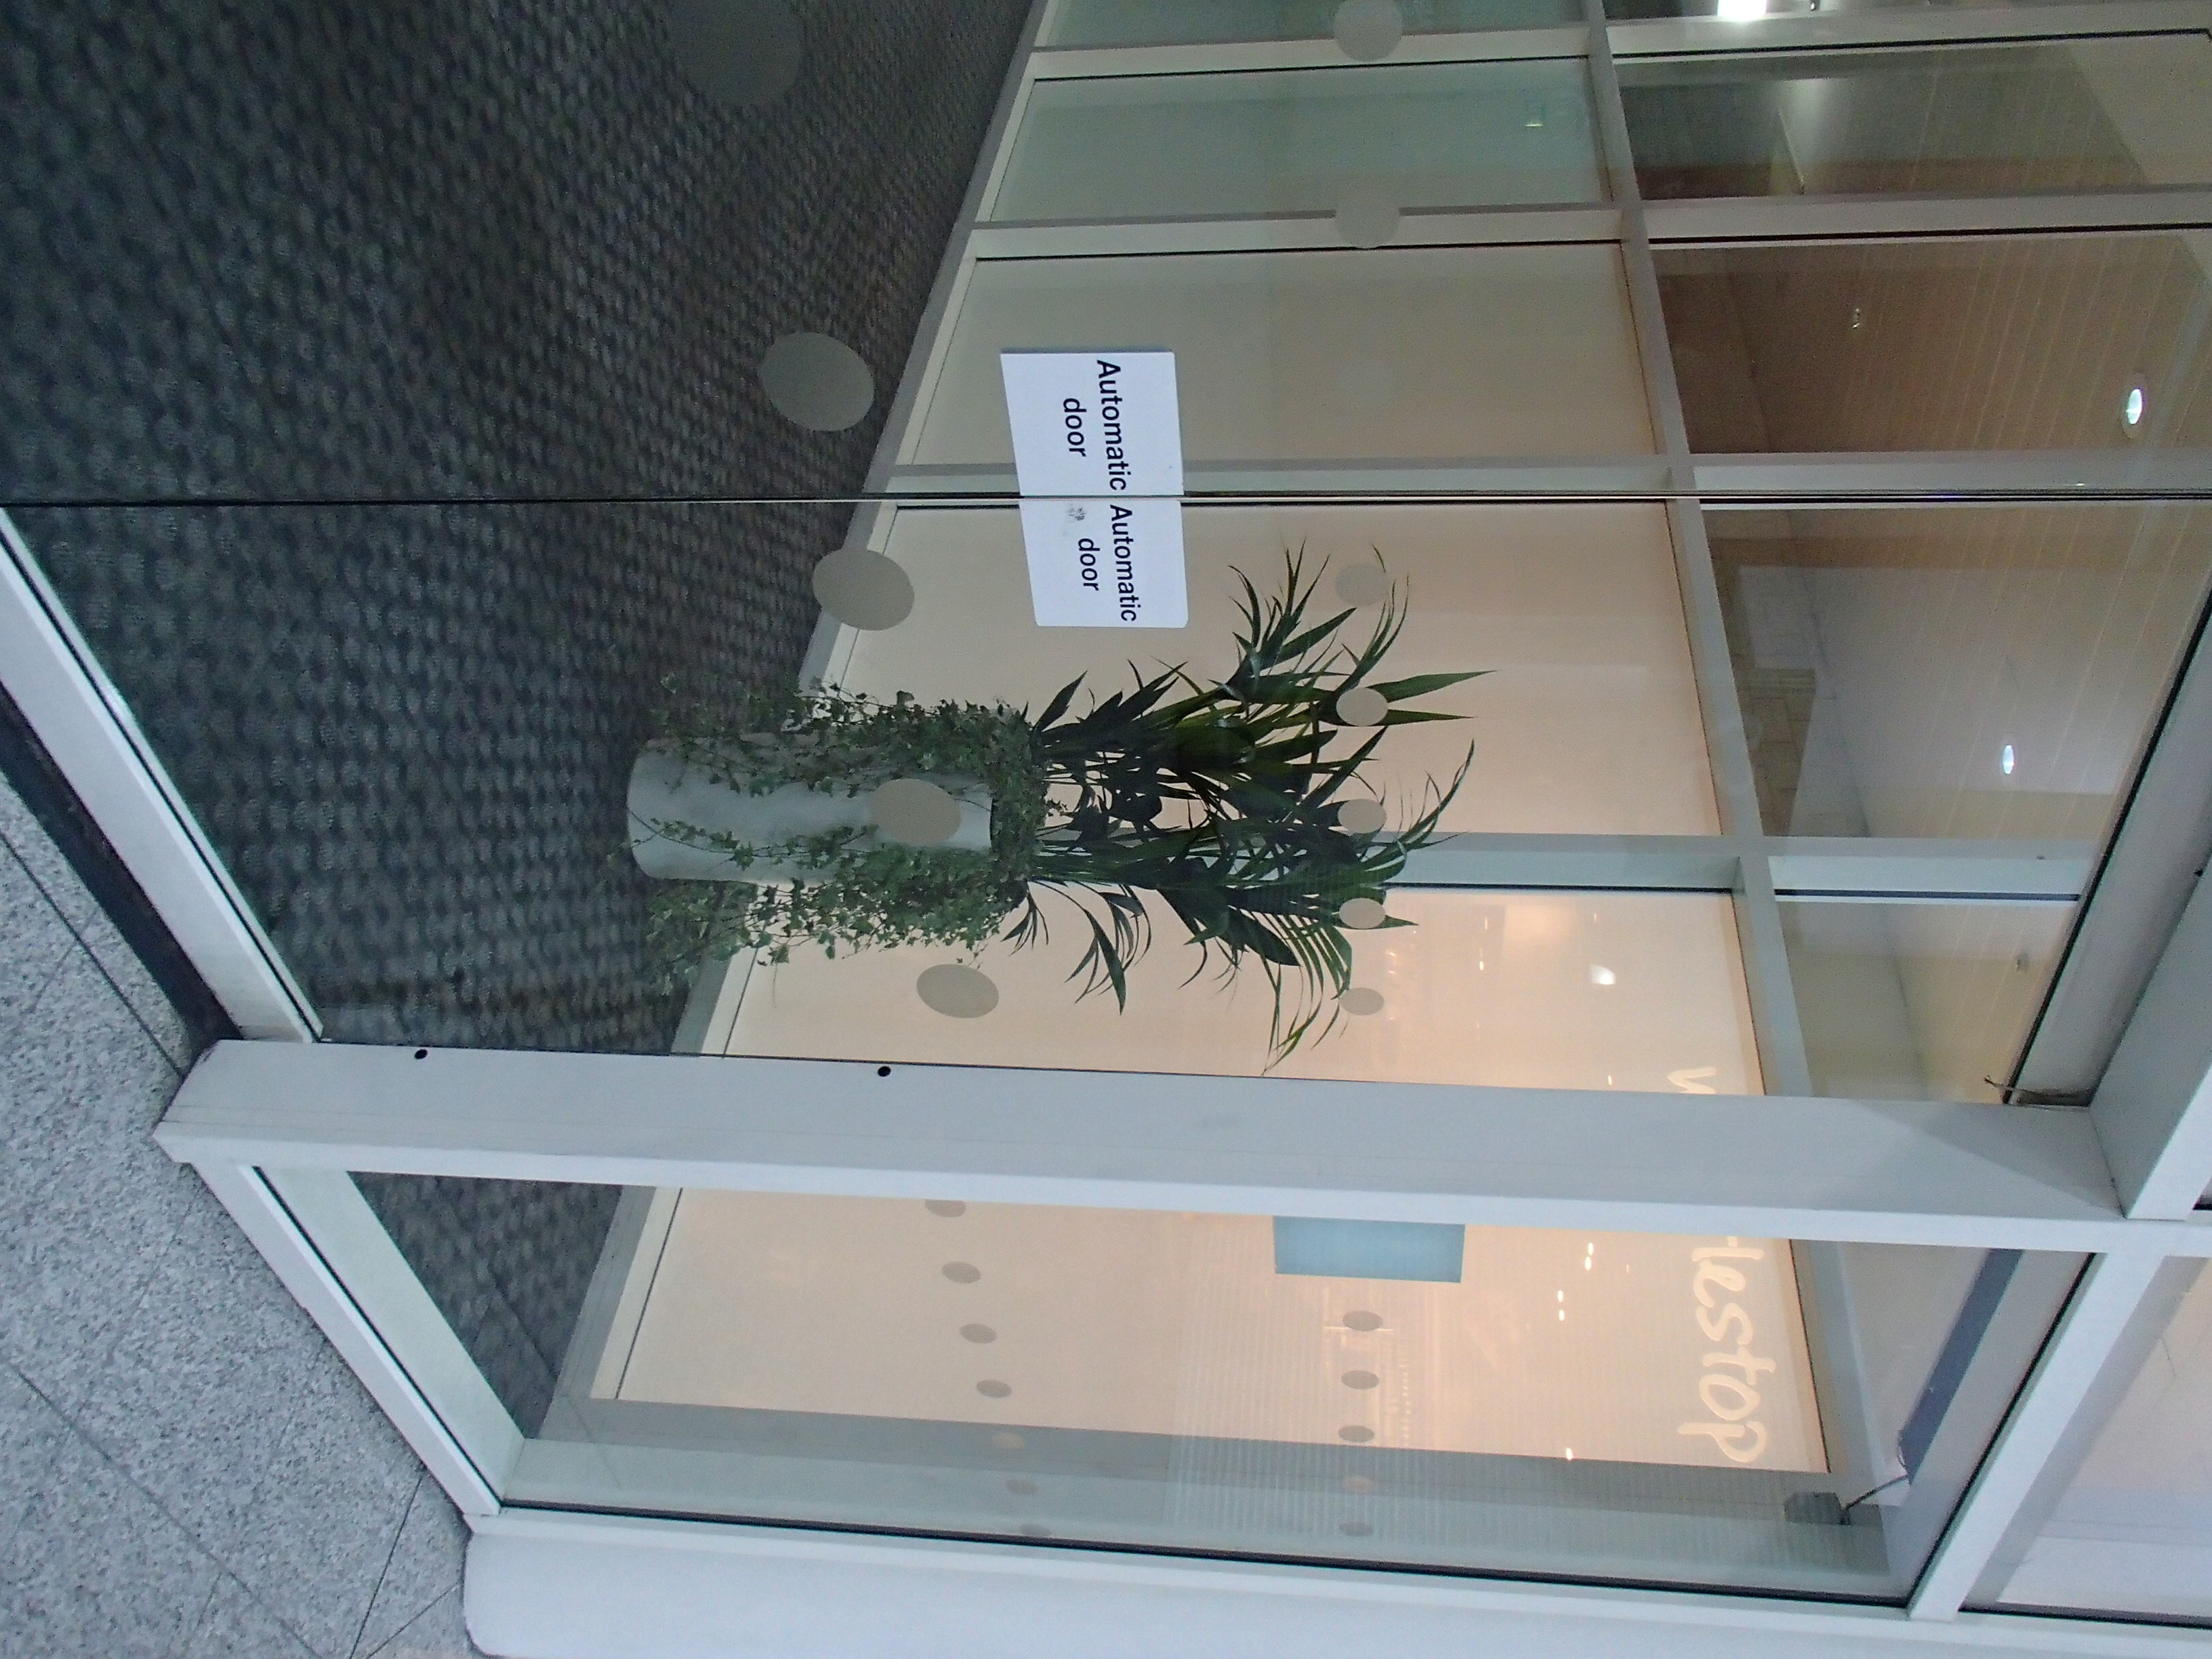
\includegraphics[width=0.5\textwidth]{figures/P1050140.JPG}
            \caption{\label{fig:pottedfern}A potted fern}
        \end{figure}
    \chapter{Plinth'd Nature}
        \begin{figure}
            \centering
            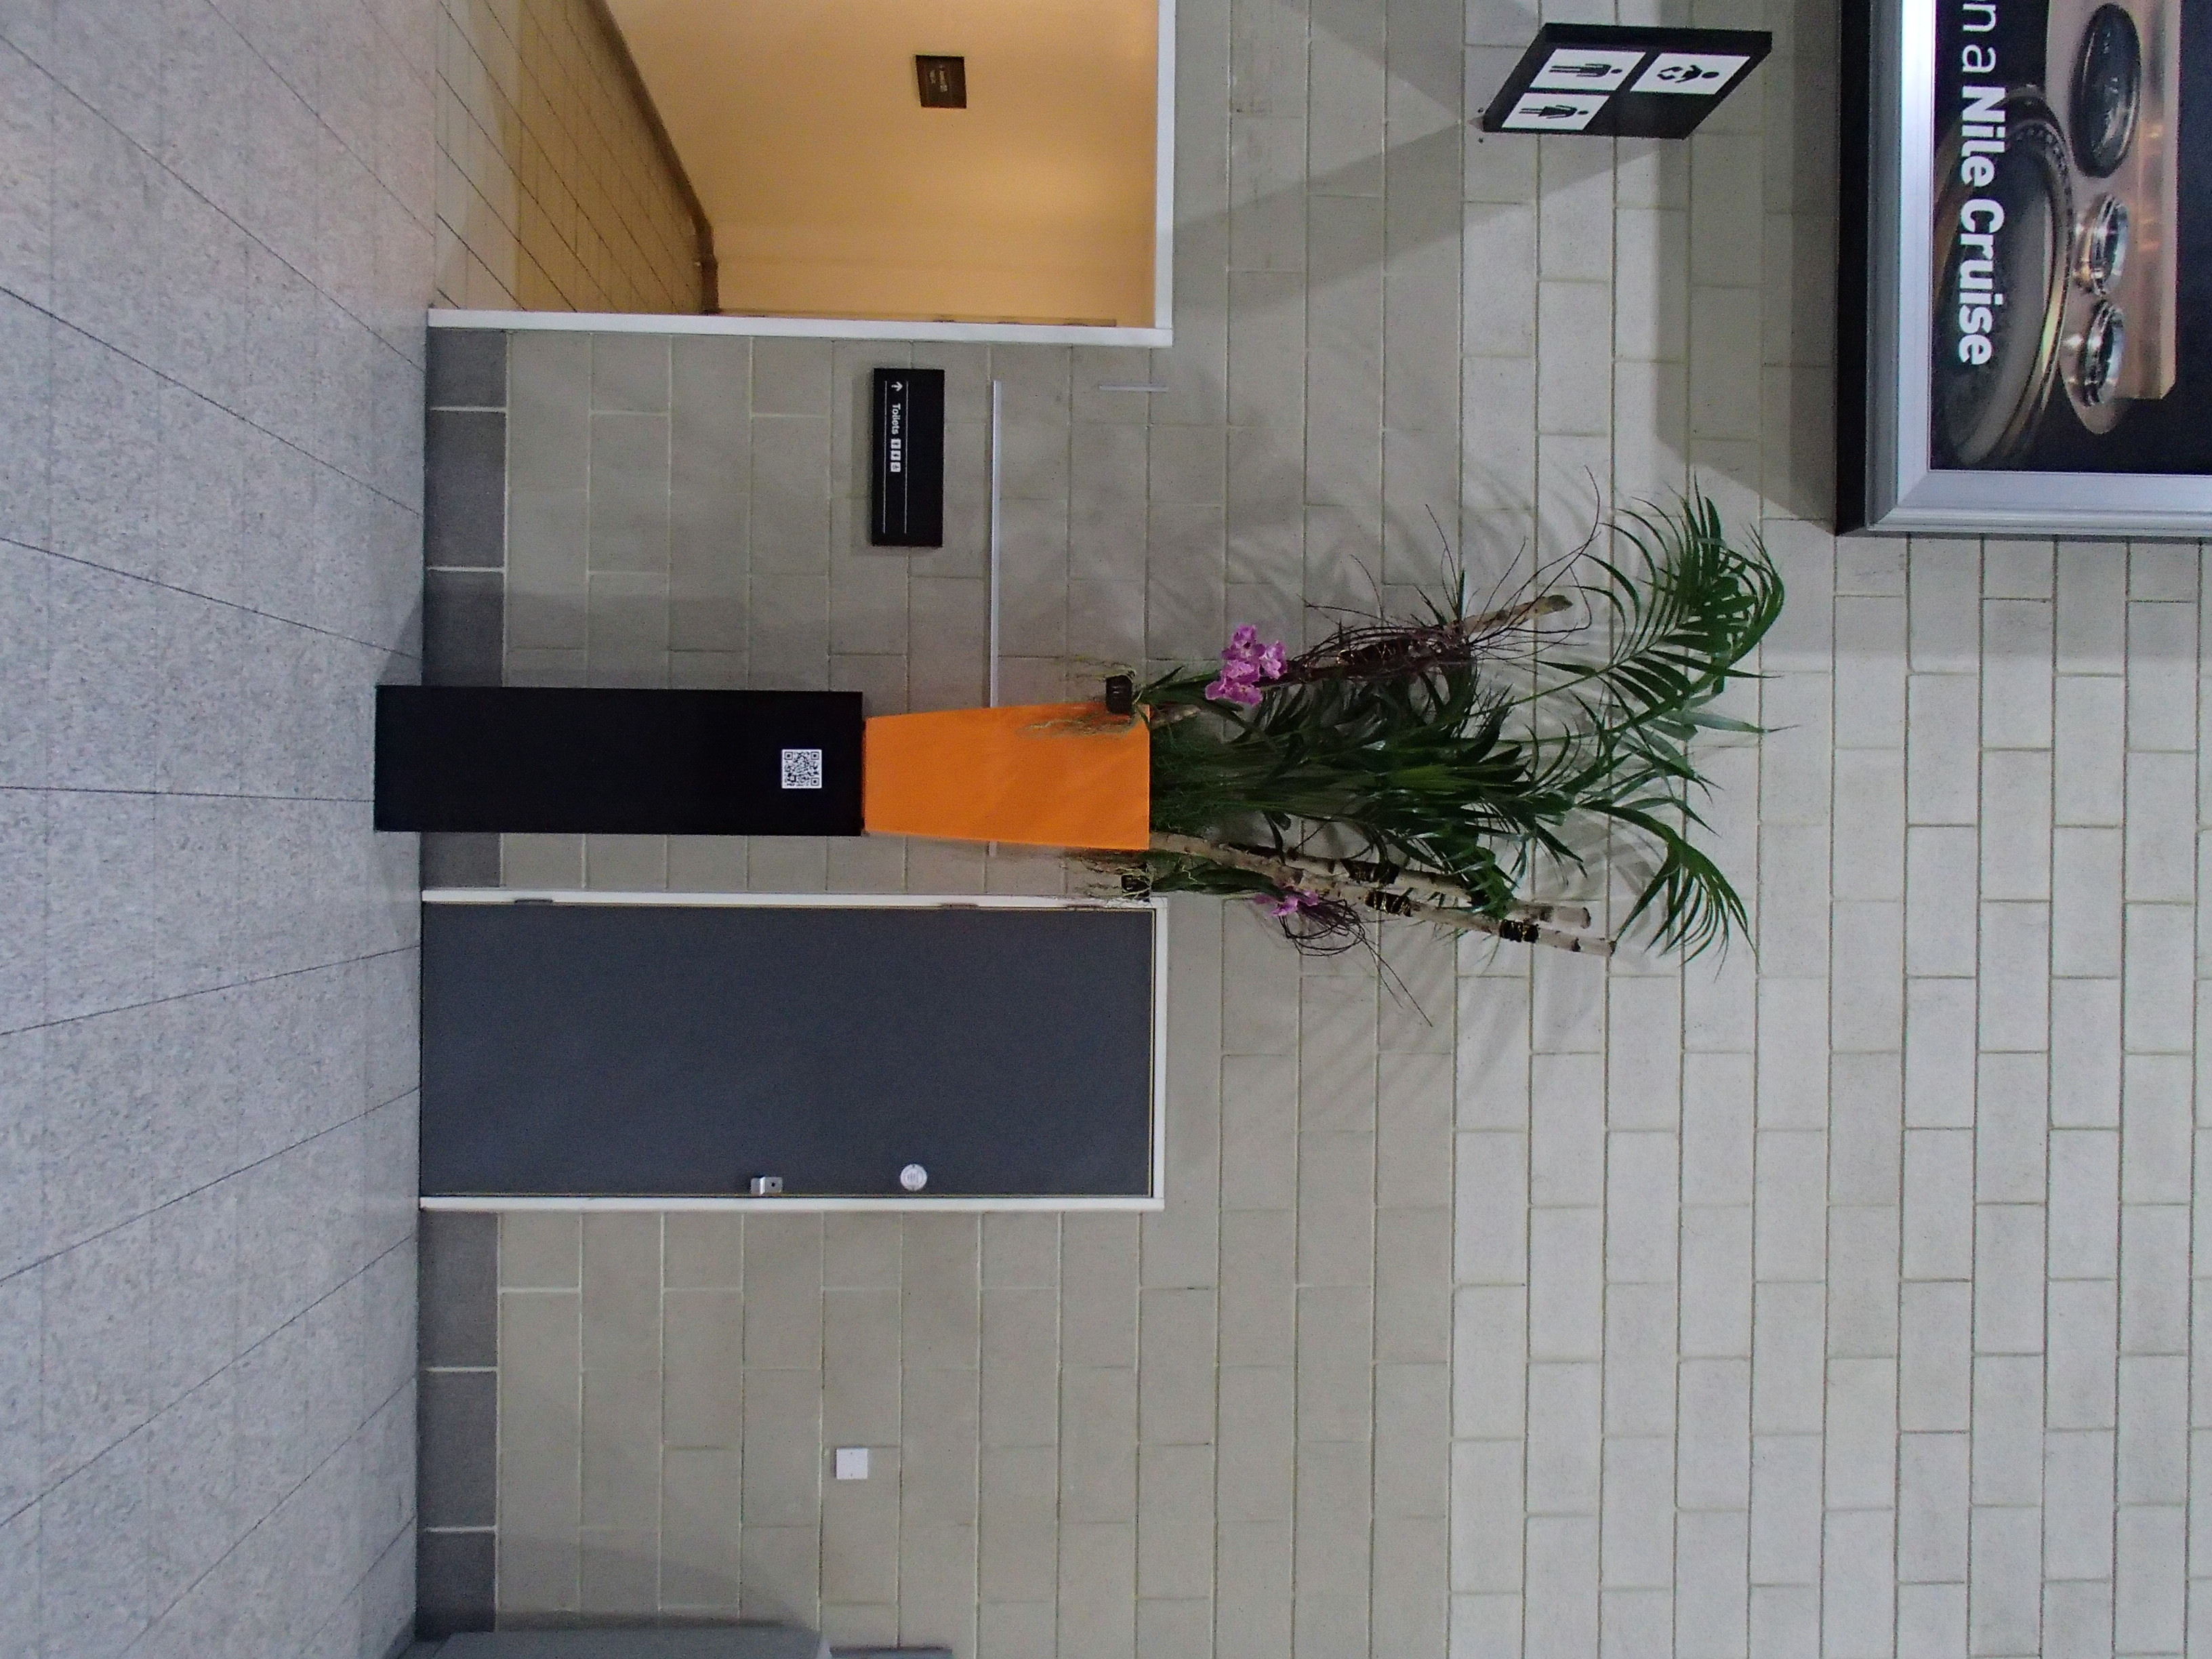
\includegraphics[width=0.5\textwidth]{figures/P1050143.JPG}
            \caption{\label{fig:pottedfern}A potted fern}
        \end{figure}
    \chapter{Nature in the 80s}
        \begin{figure}
            \centering
            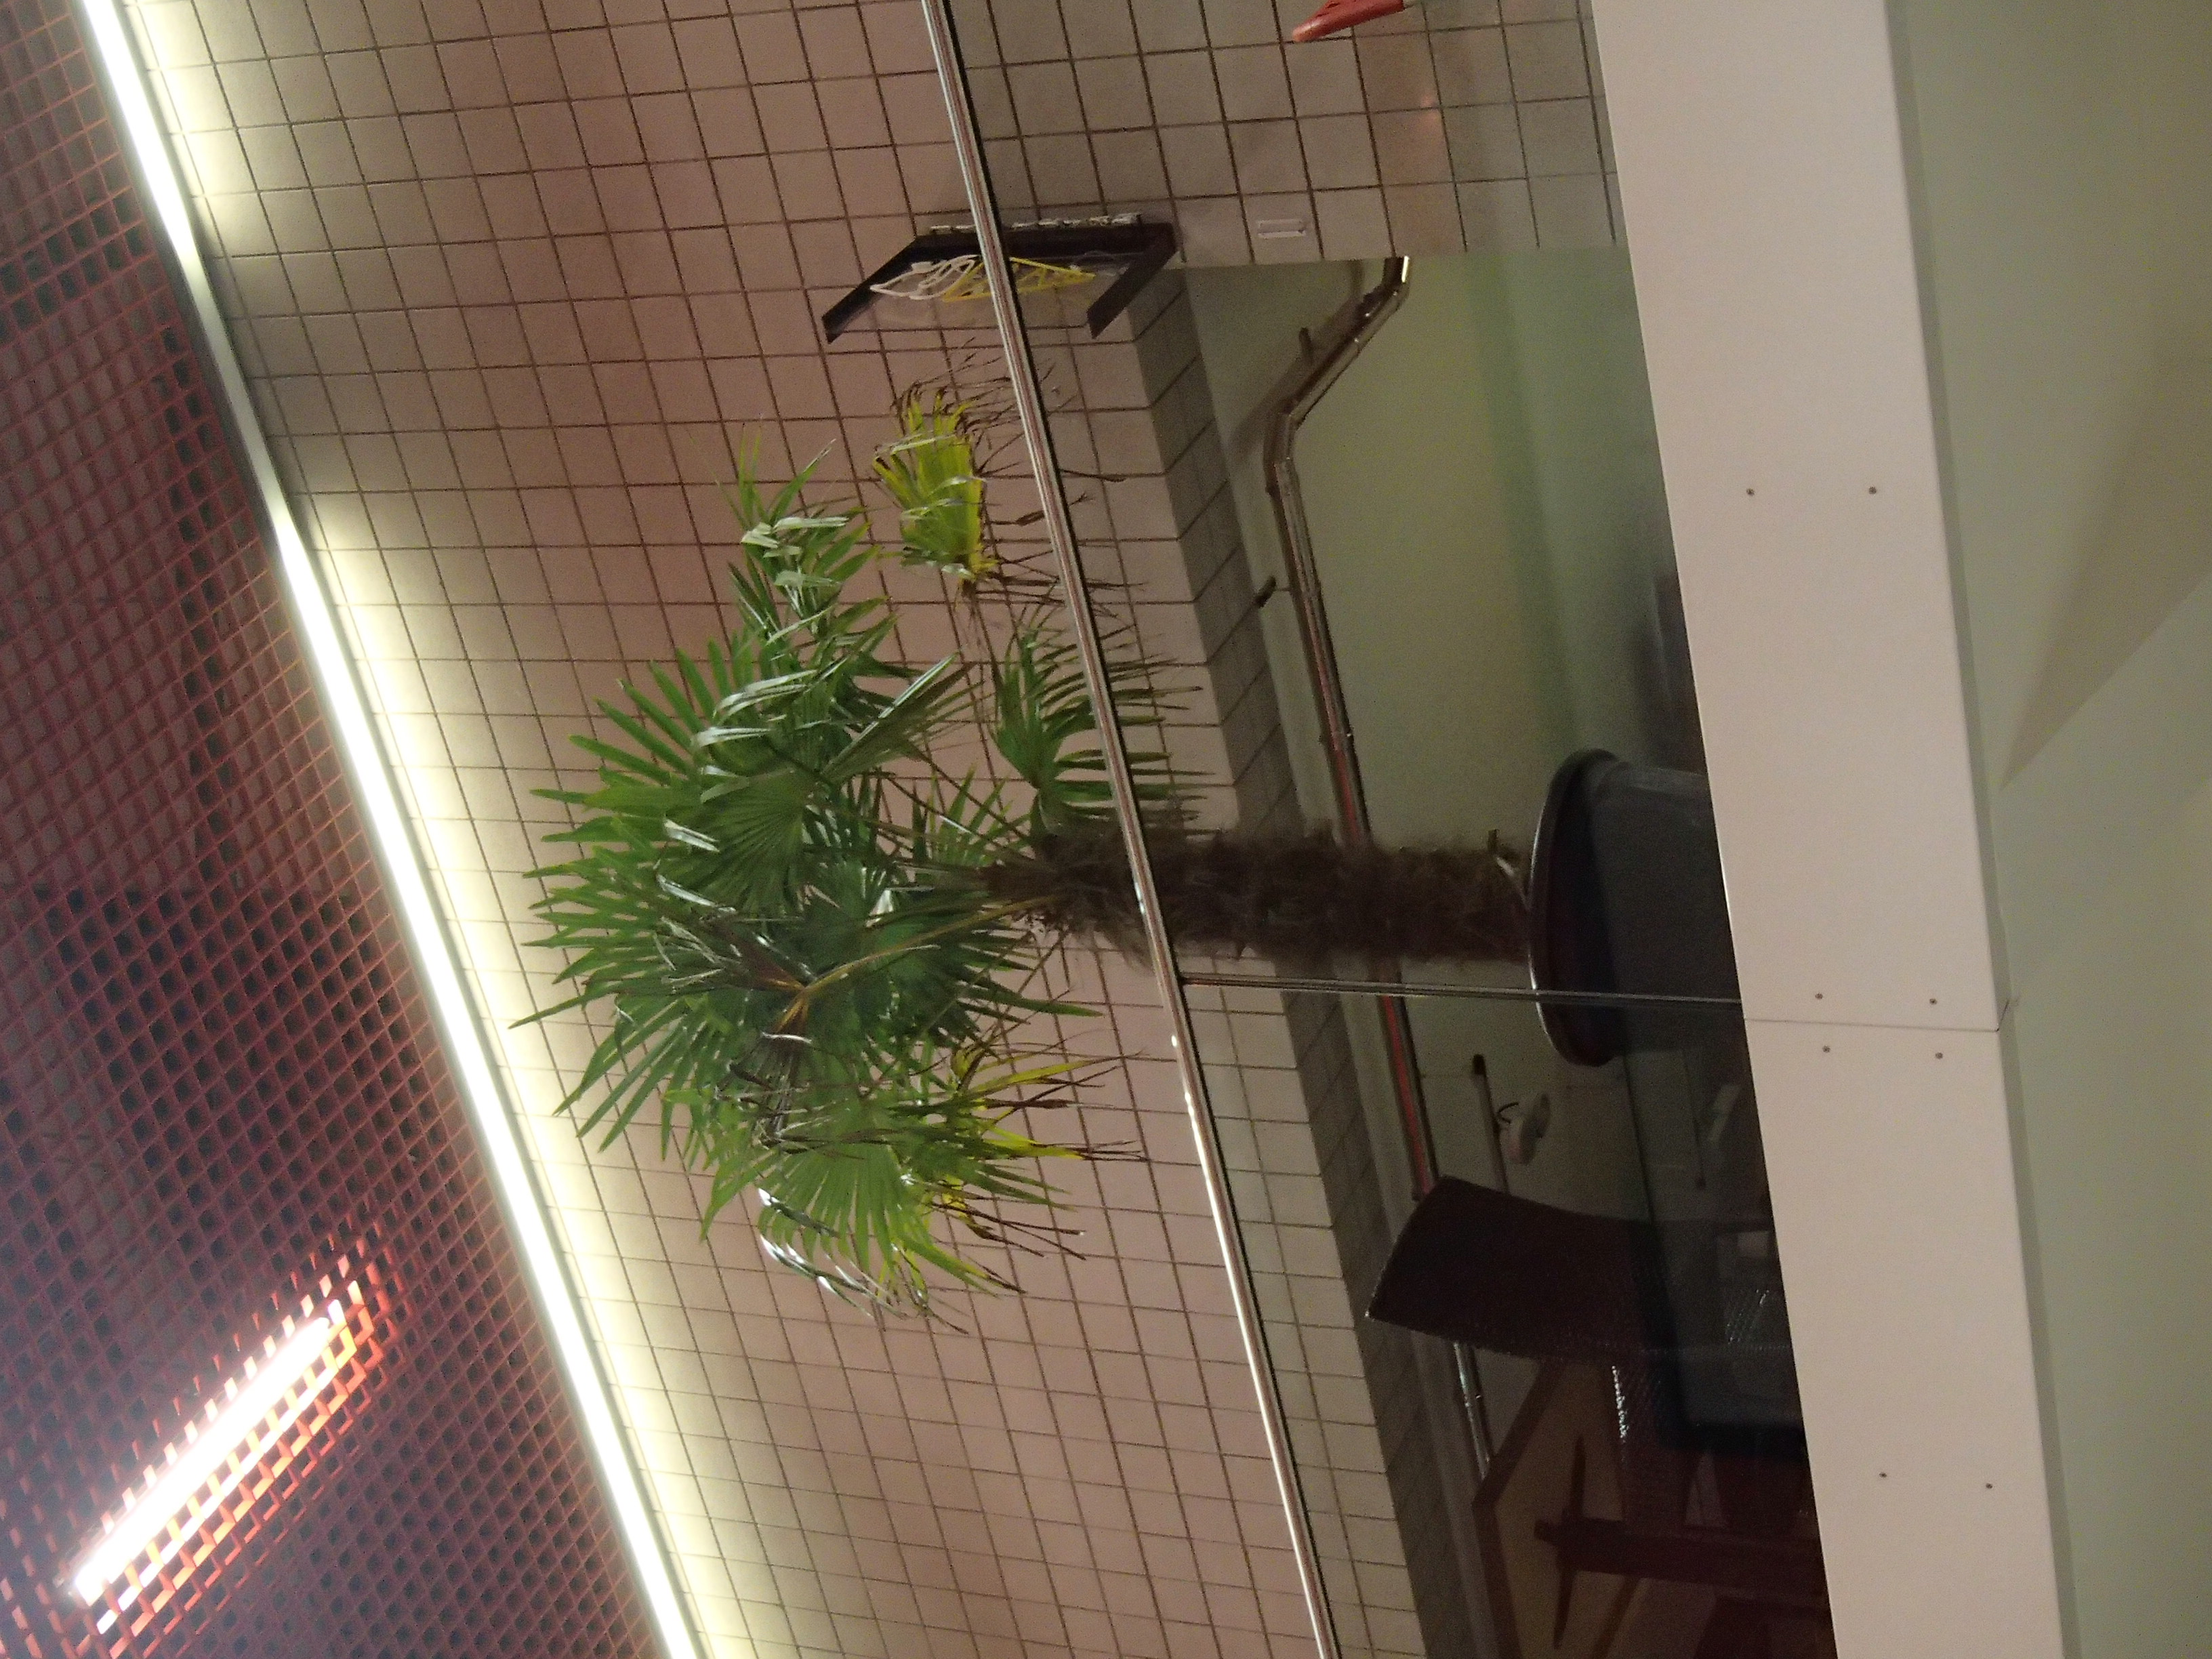
\includegraphics[width=0.5\textwidth]{figures/P1050152.JPG}
            \caption{\label{fig:pottedfern}A potted fern}
        \end{figure}
    \chapter{Cornered Nature N\textsuperscript{o}. 1}
        \begin{figure}
            \centering
            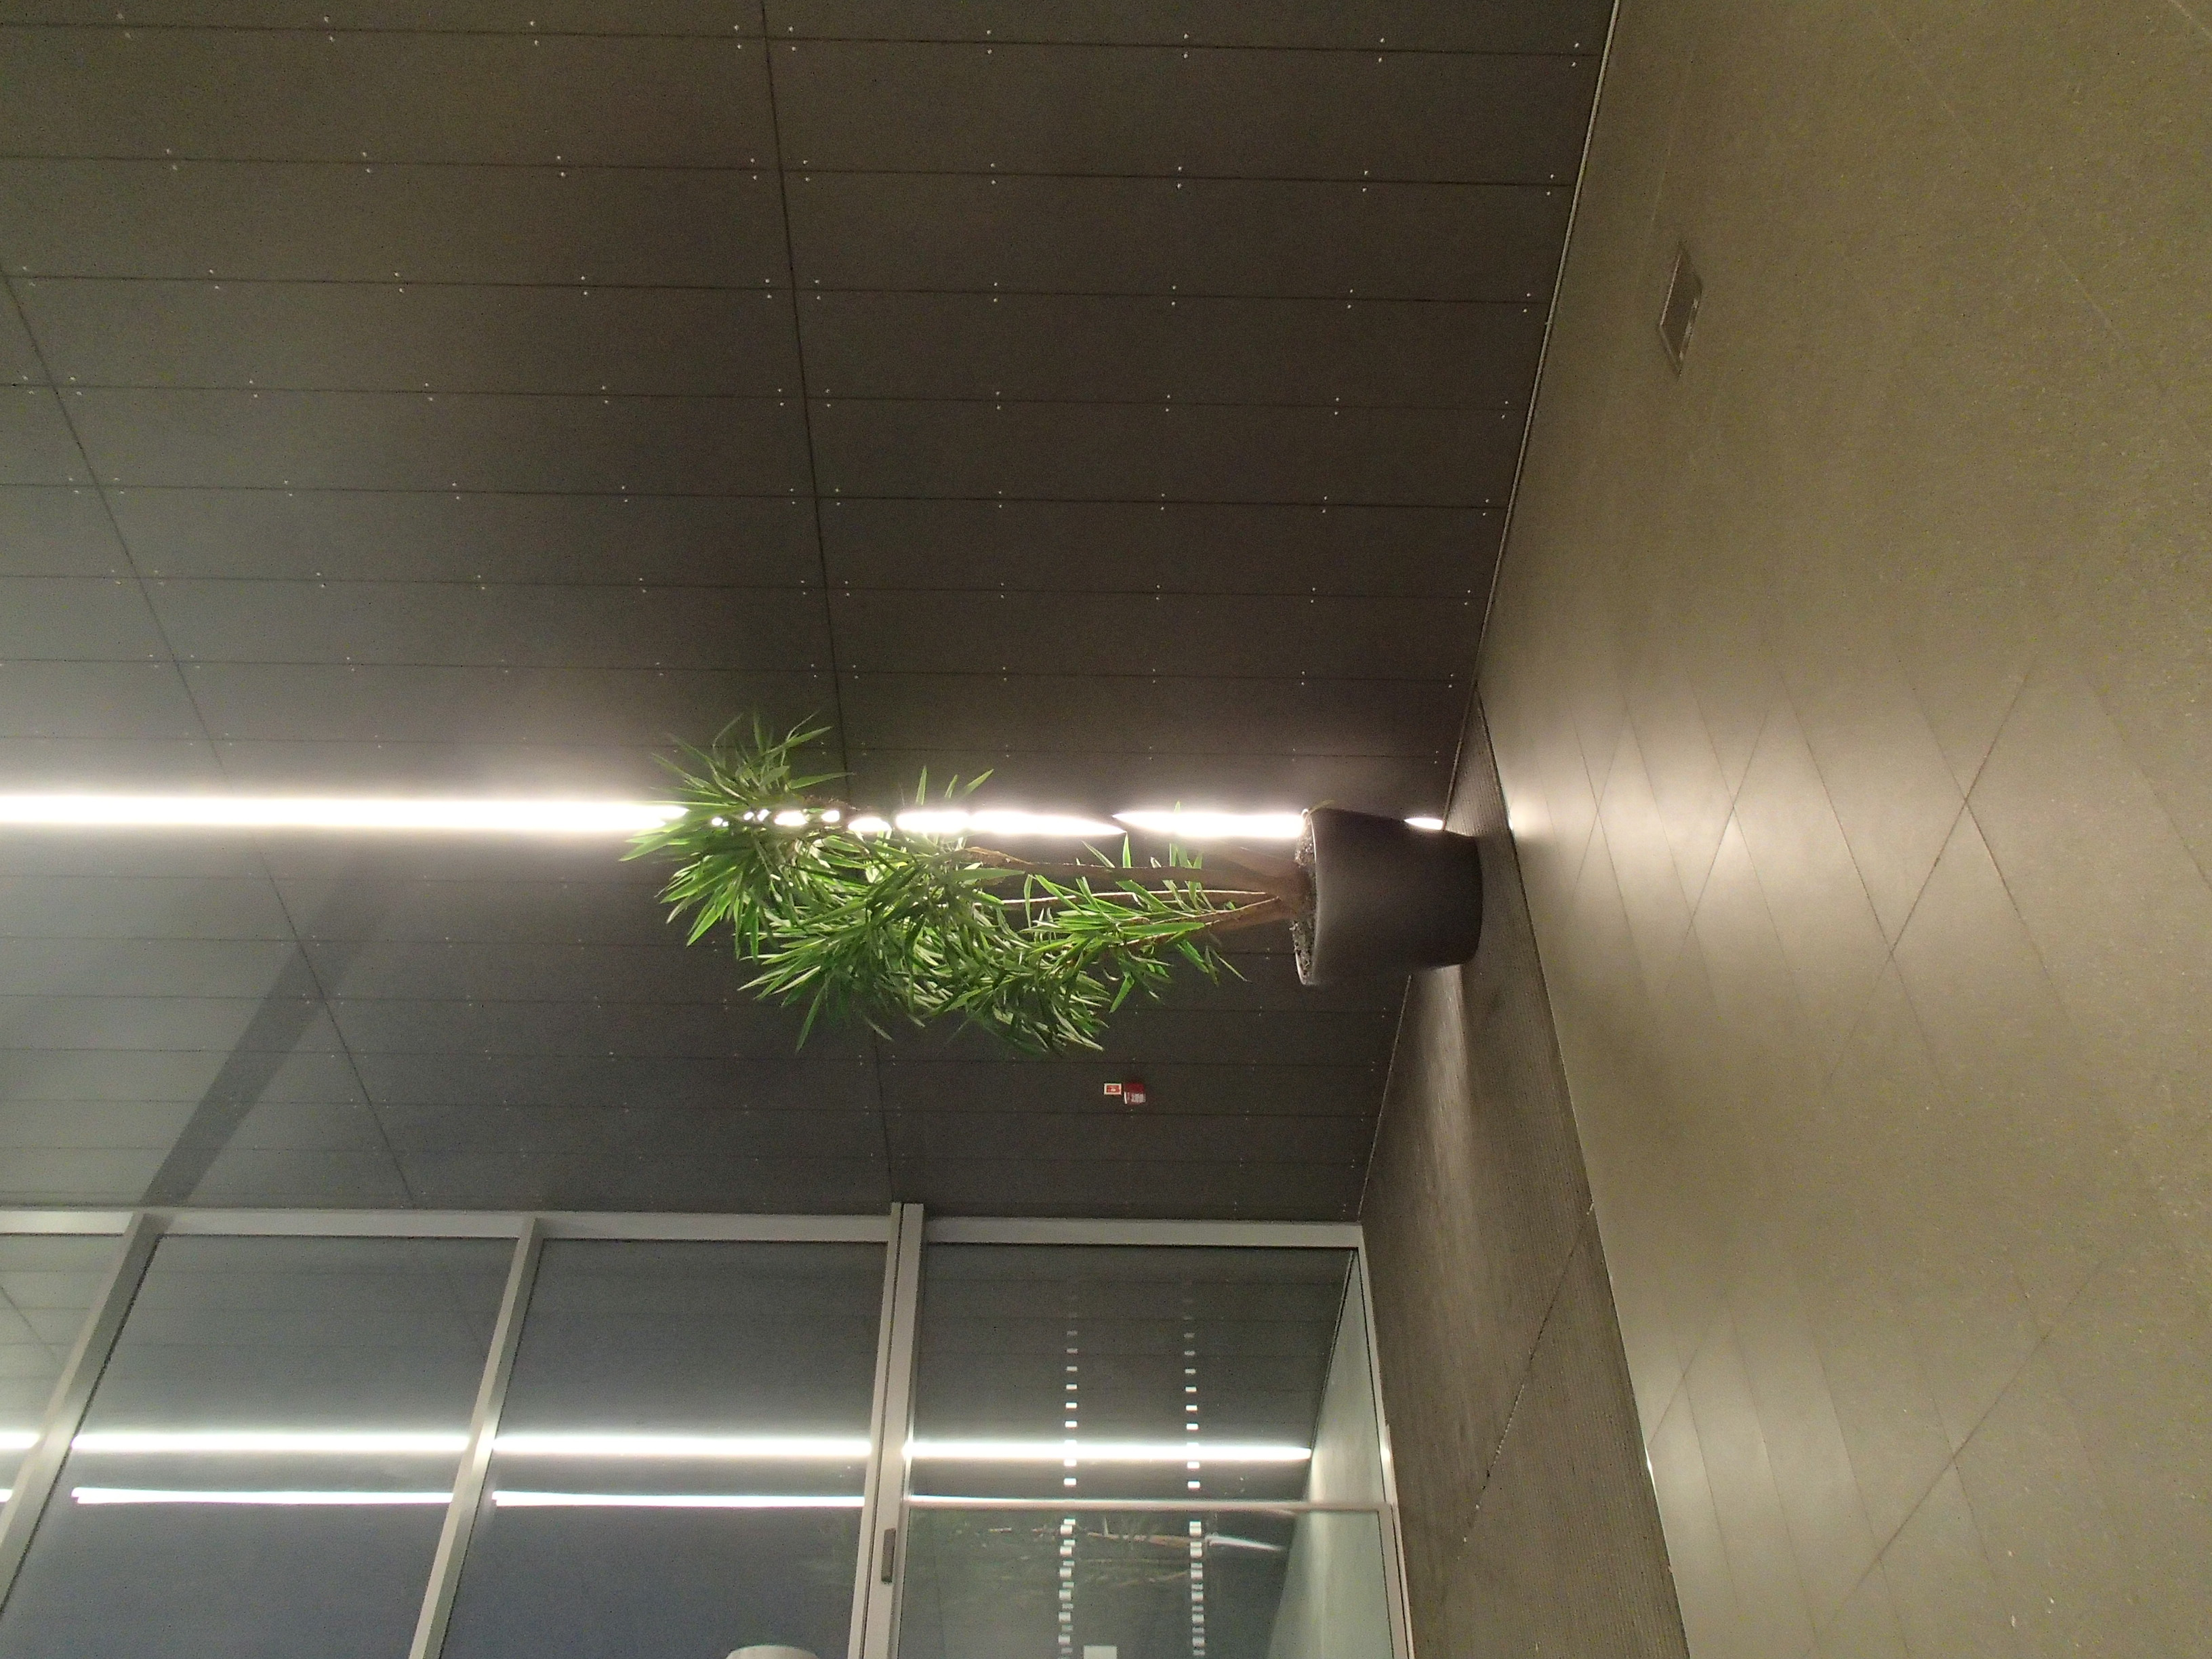
\includegraphics[width=0.5\textwidth]{figures/P1050156.JPG}
            \caption{\label{fig:pottedfern}A potted fern}
        \end{figure}
    \chapter{Cornered Nature N\textsuperscript{o}. 2}
        \begin{figure}
            \centering
            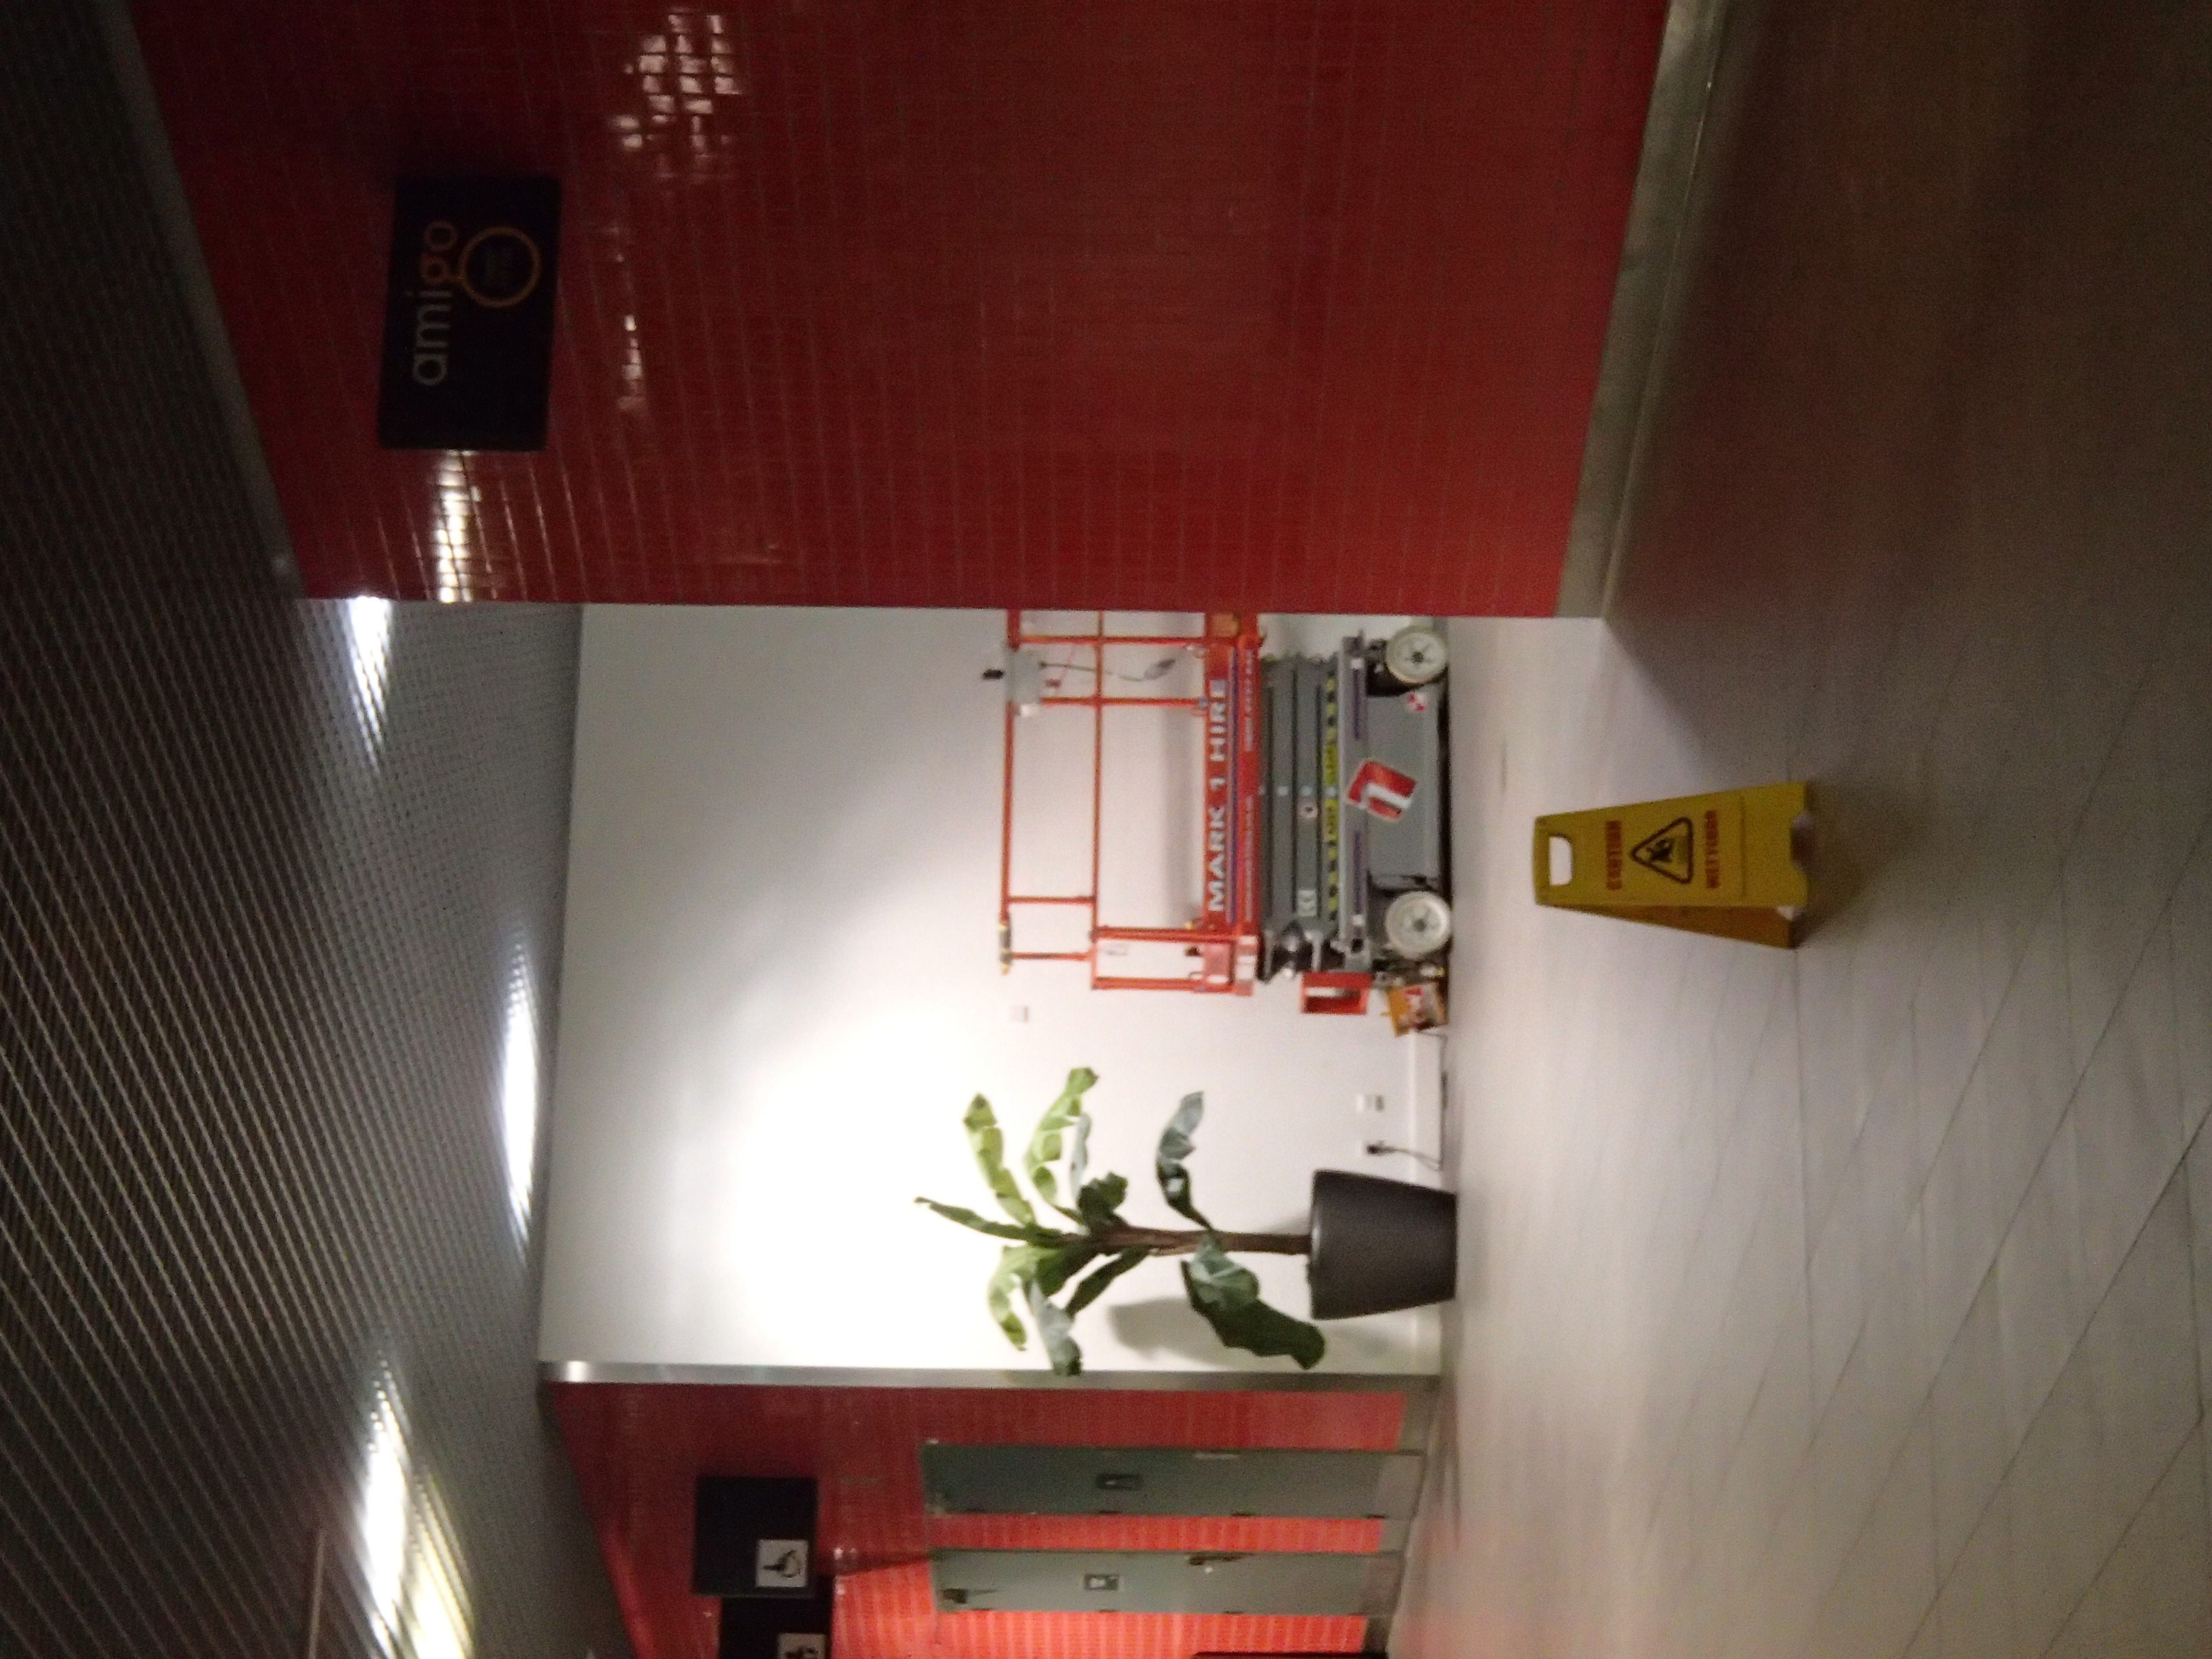
\includegraphics[width=0.5\textwidth]{figures/P1050158.JPG}
            \caption{\label{fig:pottedfern}A potted fern}
        \end{figure}
    \printindex
\end{document}
